

\documentclass{beamer}



\mode<presentation>
{
  \usetheme{Frankfurt}
  % or ...

  %\setbeamercovered{transparent}
  % or whatever (possibly just delete it)
}
\usepackage[slovene]{babel}
\usepackage[utf8]{inputenc}
%\usepackage[pdftex]{graphicx}
%\usepackage{color}
%\usepackage{float}
%\usepackage{eurosym}

\usepackage{amsfonts}
\usepackage{amsmath,amsthm}

%\usepackage[english]{babel}
% or whatever

%\usepackage[latin1]{inputenc}
% or whatever

%\usepackage{beamerthemeshadow}
\usepackage{times}
%\usepackage[T1]{fontenc}
% Or whatever. Note that the encoding and the font should match. If T1
% does not look nice, try deleting the line with the fontenc.

\newcommand{\bx}{\mathbf{x}}
\DeclareMathOperator{\Gl}{Gl}
\DeclareMathOperator{\adj}{adj}
%\newcommand{\Gl}{{\mathrm {GL}}\,}
%\newizrek{proposition}[izrek]{Proposition}

% finan�ni instrumenti
\newcommand{\PV}{\mathrm{PV}}


\newcommand{\ds}{\displaystyle}
\newcommand{\ts}{\textstyle}
\newcommand{\presledek}{\vspace{3mm}}
\newcommand{\ph}{\phantom{1}} % pomoč pri poravnavi teksta v slikah TikZ


\newcommand{\abs}[1]{ \left\lvert#1\right\rvert} 
\newcommand{\norm}[1]{\left\lVert#1\right\rVert}
\newcommand{\Co}{\operatorname{Co}} %konveksna ogrinjača

\newcommand{\R}{\mathbb R}
\newcommand{\N}{\mathbb N}
\newcommand{\Z}{\mathbb Z}
\newcommand{\C}{\mathbb C}
\newcommand{\Q}{\mathbb Q}
\newtheorem{izrek}{Izrek}
\newtheorem{lema}[izrek]{Lema}
\newtheorem{trditev}[izrek]{Trditev}
\newtheorem{posledica}[izrek]{Posledica}
\newtheorem{definicija}[izrek]{Definicija}
\newtheorem{naloga}[izrek]{Naloga}
\newtheorem{resitev}[izrek]{Naloga}
\setbeamertemplate{lema}[numbered]


\title[Računanje izotropnih vektorjev] % (optional, use only with long paper titles)
{Računanje izotropnih vektorjev}

%\subtitle
%{Presentation Subtitle} % (optional)

\author[Mirjam Pergar] % (optional, use only with lots of authors)
{\textbf{Avtor:}  Mirjam Pergar\\
\textbf{Mentor:} izred. prof. dr. Bor Plestenjak
}
% - Use the \inst{?} command only if the authors have different
%   affiliation.

\institute[Fakuleta za matematiko in fiziko] % (optional, but mostly needed)
{
%  \inst{1}%

%  \and
%  \inst{2}%
%  Department of Theoretical Philosophy\\
%  University of Elsewhere
}
% - Use the \inst command only if there are several affiliations.
% - Keep it simple, no one is interested in your street address.

\date[24. november 2015] % (optional)
{24. november 2015}

\subject{Talks}
% This is only inserted into the PDF information catalog. Can be left
% out.



% If you have a file called "university-logo-filename.xxx", where xxx
% is a graphic format that can be processed by latex or pdflatex,
% resp., then you can add a logo as follows:

% \pgfdeclareimage[height=0.5cm]{university-logo}{university-logo-filename}
% \logo{\pgfuseimage{university-logo}}



% Delete this, if you do not want the table of contents to pop up at
% the beginning of each subsection:
%\AtBeginSubsection[]
%{
%  \begin{frame}<beamer>
%    \frametitle{Outline}
%    \tableofcontents[currentsection,currentsubsection]
%  \end{frame}
%}


% If you wish to uncover everything in a step-wise fashion, uncomment
% the following command:

%\beamerdefaultoverlayspecification{<+->}
\setbeamertemplate{footline}[frame number]

\begin{document}

\begin{frame}
  \titlepage
\end{frame}

\begin{frame}
  \frametitle{Vsebina}
  \tableofcontents[pausesections]
  % You might wish to add the option [pausesections]
\end{frame}


\section{Uvod}
\subsection{Problem}
\begin{frame}
  \frametitle{Problem}
\begin{alertblock}{}
Za dano nesingularno, kvadratno $n \times n$ matriko $A$ z realnimi ali kompleksnimi elementi, nas zanima izračun enotskega vektorja $b$ z realnimi ali kompleksnimi elementi, tako da velja:
\begin{equation}\label{eq:zac}
b^\ast Ab=0.
\end{equation}
Vektor $b$, za katerega velja \eqref{eq:zac} in $b^\ast b=1$  imenujemo \textbf{izotropni vektor}. 
Bolj splošen je problem inverzne zaloge vrednosti, kjer iščemo enotski vektor $b$, za katerega velja:
\begin{equation}\label{eq:splosno}
b^\ast Ab=\mu,
\end{equation}
kjer je $\mu$ dano kompleksno število.
\end{alertblock}
\end{frame}
\begin{frame}
\begin{itemize}
\item Problem \eqref{eq:splosno} možno prevesti na problem \eqref{eq:zac} za drugo matriko, saj je \eqref{eq:splosno} enako
$$b^\ast (A-\mu I)b=0.$$
\item Če $\mu$ lastna vrednost matrike $A$, potem je rešitev pripadajoč lastni vektor matrike $A$.
\item Če $\mu$ ni lastna vrednost matrike $A$, je $A-\mu I$ nesingularna in je potreben izračun izotropnega vektorja te matrike.
\item Od sedaj naprej bomo vse vrednosti enačili z $0$.
\end{itemize}
\end{frame}
\begin{frame}
\frametitle{Zaloga vrednosti}
\begin{definicija}
\textbf{Zaloga vrednosti} matrike $A \in \C^{n\times n}$ je zaprta, konveksna podmnožica kompleksne ravnine, definirana kot
$$W(A)=\{x^\ast Ax: x \in \C^n, x^\ast x=1\}.$$
\end{definicija}\pause
Očitno je zaloga vrednost $W(A)$ množica vseh Rayleighovih kvocientov matrike $A$. Če hočemo, da ima \eqref{eq:zac} vsaj eno rešitev, mora biti izhodišče v $W(A)$. Označimo s $\sigma(A)$ množico vseh lastnih vrednosti matrike A, ki jo imenujemo spekter.
\end{frame}
\begin{frame}
\frametitle{Lastnosti zaloge vrednosti}
\begin{enumerate}
\item $W(A)$ je konveksna, zaprta in omejena.
\item $\sigma(A)\subseteq W(A).$
\item Za vsako unitarno matriko $U$ je $W(U^\ast AU)=W(A).$
\item $W(A+zI)=W(A)+z$ in $W(zA)=zW(A)$ za vsako kompleksno število $z$.
\item Rob zaloge vrednosti $W(A), \partial W(A)$ je kosoma algebrska krivulja, in vsaka točka v kateri $\partial W(A)$ ni diferenciabilna je lastna vrednost matrike $A$.
\item Če je $A$ normalna, potem $W(A)=\Co(\sigma(A))$, kjer s $\Co$ označimo zaprto konveksno ogrinjačo množice.
\item $W(A)$ je daljica na realni osi, če in samo če je $A$ hermitska.
\end{enumerate}
\end{frame}
\begin{frame}
\begin{izrek}
Naj imata $A$ in $b$ realne ali kompleksne elemente. Potem veljajo enakosti:
$$b^\ast Ab=0\Leftrightarrow b^\ast (A+A^\ast)b=0 \ \textrm{in}\  b^\ast(A-A^\ast)b=0.$$
\end{izrek}\pause
\begin{itemize}
\item Če velja le $b^\ast (A+A^\ast)b=0 \Rightarrow \Re(b^\ast Ab)=0$.
\item Če velja le $b^\ast(A-A^\ast)b=0 \Rightarrow \Im(b^\ast Ab)=0$.
\item Ko sta $b$ in $A$ realna, je problem mnogo enostavnejši, saj moramo upoštevati le simetričen del matrike $A$.
\end{itemize}
\end{frame}
\begin{frame}
\begin{lema} %\cite{lipkin}
Izotropni vektorji matrike A so identični izotropnim vektorjem njenega simetričnega dela.
\end{lema} \pause
Velja enakost:
\begin{block}{}
$$b^T Ab=0 \Leftrightarrow b^T (A+A^T)b=0.$$ 
\end{block}
\begin{itemize}
\item Hermitski del matrike $A$ bomo označili s $H=(A+A^\ast)/2$.
\item Poševno-hermitski del matrike $A$ bomo označili z $\tilde{K}=(A-A^\ast)/2=\imath K$.
\end{itemize}
\end{frame}
\subsection{Uporaba}
\begin{frame}
\frametitle{Uporaba}
\begin{itemize}
\item Preučevanje delne stagnacije GMRES algoritma za reševanje linearnih sistemov z realnimi matrikami.
\item Preučevanje konvergence nekaterih iterativnih metod za reševanje linearnih sistemov.
\item Aplikacije v numerični analizi, diferencialnih enačbah, teoriji sistemov itd.
\end{itemize}
\end{frame}
\section{Realne matrike}
\subsection{Uvod}
\begin{frame}
\frametitle{Realne matrike}
\begin{block}{}
Ko je $A$ realna matrika, nas zanima kako izračunati rešitev naslednje enačbe:
\begin{equation}\label{eq:realna}
b^\ast Hb=0,
\end{equation}
kjer je $H$ realna in simetrična matrika (t.j. $H=H^T$).
\end{block}\pause
Vemo:
\begin{itemize}
\item $W(A)$ simetrična glede na realno os.
\item $0 \in W(A)$, če in samo če $\lambda_n\le0\le\lambda_1$, kjer sta $\lambda_n$ in $\lambda_1$ najmanjša in največja lastna vrednost matrike $H$.
\end{itemize}
\end{frame}
\begin{frame}
Naj bosta $x_1$ in $x_n$ realna lastna vektorja, pripadajoča $\lambda_1$ in $\lambda_n$.Potem sta:
\begin{itemize}
\item $x_1^T Ax_1=x_1^T Hx_1=\lambda_1$.
\item $x_n^T Ax_n=x_n^T Hx_n=\lambda_n$.
\end{itemize}
realni točki na skrajni levi in skrajni desni zaloge vrednosti $W(A)$ na realni osi.
\begin{itemize}\pause
\item Realne rešitve \eqref{eq:realna} izračunamo z uporabo lastnih vektorjev matrike $H$. 
\item Predpostavimo, da iščemo vektorje $b$ z normo 1.\pause
\item $H$ zapišemo kot $$H=X\Lambda X^T,$$ kjer je $\Lambda$ matrika, ki ima na diagonali lastne vrednosti $\lambda_i$, ki so realna števila in $X$ je ortogonalna matrika lastnih vektorjev, tako da $X^T X=I$.
\end{itemize}
\end{frame}
\begin{frame}
\begin{itemize}
\item Uporabimo ta spektralni razcep v \eqref{eq:realna}: $$b^\ast Hb=b^\ast X\Lambda X^T b=0.$$ 
\item  Označimo s $c=X^Tb$ vektor projekcije $b$ na lastne vektorje matrike $H$. 
\end{itemize}\pause
\begin{izrek} \label{izrek2}
Naj bo $b$ rešitev problema \eqref{eq:realna}. Potem vektor $c=X^T b$ s komponentami $c_i$ zadošča naslednjima enačbama:
\begin{align}
\sum_{i=1}^{n} \lambda_i \abs{c_i}^2=0 \label{eq:en1},\\
\sum_{i=1}^{n}\abs{c_i}^2=1. \label{eq:en2}
\end{align}
\end{izrek}
\end{frame}
\subsection{Iskanje izotropnih vektorjev}
\begin{frame}
\frametitle{Iskanje izotropnih vektorjev}
\begin{block}{}
Če predpostavimo, da nimajo vse lastne vrednosti $H$ enakega predznaka, potem more za najmanjšo lastno vrednost $\lambda_n$ veljati $\lambda_n <0$. 
 Naj bo $k>1$ tak, da je $\lambda_k >0$ in $0<t<1, t\in \R$ .  Označimo $\abs{c_n}^2 =t$,$\abs{c_k}^2=1-t$ in $c_i \not =0, i\not=n,k$, kar velja zaradi enačbe \eqref{eq:en2}, $t+ (1-t)=1$. Iz \eqref{eq:en1} mora veljati enačba: $$\lambda_n t +\lambda_k (1-t)=0,$$ katere rešitev je:
\begin{equation}
t_s=\frac{\lambda_k}{\lambda_k -\lambda_n}.
\end{equation}
\end{block}
\end{frame}
\begin{frame}
\begin{itemize}
\item Absolutna vrednost $c_1$ (oz. $c_k$) je kvadratni koren od $t_s$ (oz. $1-t_s$).\pause
\item Ker je $b=Xc$, sta dve realni rešitvi: $$b_1=\sqrt{t_s}x_n +\sqrt{1-t_s}x_k,\quad b_2=-\sqrt{t_s}x_n+\sqrt{1-t_s}x_k,$$ kjer sta $x_1$ in $x_k$ lastna vektorja pripadajoča  $\lambda_n$ in $\lambda_k$.\pause
\item Ker imata izraza v rešitvah enaka imenovalca, lahko rešitvi zapišemo kot: $$b_1=\sqrt{\lambda_k}x_n+\sqrt{\abs{\lambda_n}}x_k, \quad b_2=-\sqrt{\lambda_k}x_n+\sqrt{\abs{\lambda_n}}x_k$$.\pause
%(sledi iz \cite{lipkin}).
\item Vektor mora biti normiran:
\begin{align*}
b_1=\sqrt{\frac{\lambda_k}{\lambda_k +\abs{\lambda_n}}}x_n + \sqrt{\frac{\abs{\lambda_n}}{\lambda_k +\abs{\lambda_n}}}x_k,\\ b_2=-\sqrt{\frac{\lambda_k}{\lambda_k +\abs{\lambda_n}}}x_n + \sqrt{\frac{\abs{\lambda_n}}{\lambda_k +\abs{\lambda_n}}}x_k.
\end{align*}
\end{itemize}
\end{frame}
\begin{frame}
\frametitle{Število rešitev}
Uporabimo lahko vsak par pozitivnih in negativnih lastnih vrednosti. Ta postopek lahko vrne toliko rešitev kot je dvakratno število parov lastnih vrednosti matrike $H$ z nasprotnimi predznaki, če so vse lastne vrednosti različne. Predpostavimo, da je $b$ realen.\pause
\begin{posledica}%\cite{lipkin}
Dobljena izotropna vektorja sta ortogonalna ($b_1 ^T b_2=0$), če in samo če $\lambda_k=-\lambda_n$.
\end{posledica}\pause
Ko sta $A$ in $b$ realna smo dokazali naslednji izrek:
\begin{izrek}
Če je $A$ realna in nedefinitna (t.j. ni pozitivno in negativno definitna), potem obstajata najmanj dva neodvisna realna izotropna vektorja.
\end{izrek}
\end{frame}
\begin{frame}
\frametitle{Neskončno rešitev}
\begin{itemize}
\item Pokazati želimo, da imamo neskončo število realnih rešitev in jih izračunati. \pause
\item Potrebujemo vsaj 3 različne lastne vrednosti z različnimi predznaki.\pause
\item Predpostavimo, da $\lambda_1 <0<\lambda_2<\lambda_3$.\pause
\item Naj bo $t_1=\abs{c_1}^2$, $t_2=\abs{c_2}^2$.\pause
\item Veljati mora enačba \eqref{eq:en2}
\begin{equation*}%\label{trije}
\lambda_1 t_1 +\lambda_2 t_2 +\lambda_3 (1- t_1 -t_2)=(\lambda_1 -\lambda_3)t_1 +(\lambda_2 -\lambda_3)t_2 +\lambda_3=0,
\end{equation*}
s pogoji: $t_i \ge 0, i=1,2$ in $t_1 +t_2\le1$.
\end{itemize}
\end{frame}
\begin{frame}
\frametitle{Neskončno rešitev}
\begin{itemize}
\item Dobimo premico definirano v $(t_1,t_2)$ ravnini 
\begin{block}{}
$$t_2=\frac{\lambda_3}{\lambda_3 - \lambda_2} -\frac{\lambda_3 -\lambda_1}{\lambda_3 -\lambda_2}t_1.$$
\end{block}\pause
\item Pogoji za $t_1,t_2$ definirajo trikotnik.
\item Potrebno je preveriti, če premica seka trikotnik.\pause
\item $t_1$-os seka pri $\lambda_3 /(\lambda_3 -\lambda_1)>1$.
\item $t_2$-os seka  pri $\lambda_3 /(\lambda_3 - \lambda_2)<1$.\pause
\item Vse dopustne vrednosti za $t_1$ in $t_2$ so dane z daljico v trikotniku. 
\item Zato obstaja neskončno število možnih pozitivnih parov $(t_1,t_2)$.
\end{itemize}
\end{frame}
\begin{frame}
\frametitle{Zgled}
Poglejmo zgled, ko imamo lastne vrednosti $\lambda_1=-1, \lambda_2=2$ in $\lambda_3=2$. Enačba premice je $t_2=2-3t_1$.
\begin{center}
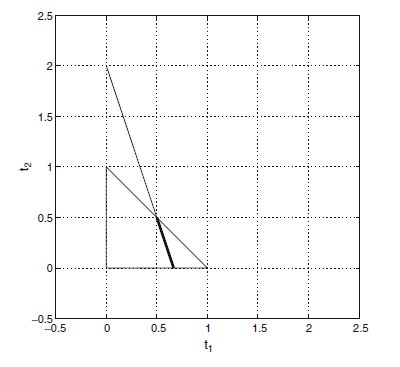
\includegraphics[width=5cm]{trikotnik.jpg}
\end{center}
\end{frame}
\begin{frame}
\frametitle{Neskončno rešitev}
Ta problem za iskanje koeficientov je v treh dimenzijah in možne rešitve $t$-ja so v eni dimenziji. Takšna konstrukcija pripelje do naslednjega izreka:
\begin{izrek}
Če je $n>2$ in $A$ je realna in nedefinitna, ima matrika $H$ vsaj tri različne lastne vrednosti z različnimi predznaki. Potem obstaja neskončno število realnih izotropnih vektorjev.
\end{izrek}\pause
\begin{block}{Splošen zapis}
\begin{equation*}
\sum_{i=1}^{k-1} (\lambda_i -\lambda_k)t_i +\lambda_k =0, \quad t_i\ge0, i=1, \dots,k-1, \sum_{i=1}^{k-1}t_i \le1.
\end{equation*}
\end{block}
\end{frame}
\section{Kompleksne matrike}
\subsection{Uvod}
\begin{frame}
\frametitle{Kompleksne matrike}
Predstavljene bodo grobe ideje algoritmov naslednjih avtorjev:
\begin{enumerate}
\item \emph{Meurant}.
\item \emph{Carden}.
\item \emph{Chorianopoulos, Psarrakos in Uhlig}.
\end{enumerate}
\end{frame}
\subsection{Iskanje izotropnih vektorjev}
\subsubsection{Meurant 1.}
\begin{frame}
\frametitle{Meurant 1.}
\begin{itemize}
\item V nekaterih primerih lahko izračunamo rešitve s samo enim ra\-ču\-na\-njem lastnih vrednosti in vektorjev matrike $K$.\pause
\item Uporabimo lastne vektorje matrike $H$.\pause
\item Če ima matrika $A$ kompleksne elemente, nam prejšnja konstrukcija za realne matrike vrne le vektorje za katere je $\Re(b^\ast Ab)=0$.\pause
\item Z uporabo treh lastnih vektorjev $H$, obstaja neskončno rešitev dobljenih na daljici v trikotniku omejitev.\pause
\item  Če sta imaginarna dela, ki ustrezata robnima točkama daljice, različnih predznakov, potem iz izreka o povprečni vrednosti sledi, da obstaja točka na daljici, ki ima ničeln imaginarni del.
\end{itemize}
Opomba: to vsebuje samo izračun kvadratne forme $x^\ast Ax$. Ne potrebujemo nobenih izračunov lastnih vrednosti in vektorjev.
\end{frame}
\subsubsection{Meurant 2.}
\begin{frame}
\frametitle{Meurant 2.}
\begin{itemize}
\item Uporabimo lastne vrednosti in lastne vektorje matrike $K=(A-A^\ast)/(2i)$, ki je hermitska. 
\item S kombiniranjem lastnih vektorjev matrike $K$ pripadajočim k pozitivnim in negativnim lastnim vrednostim, lahko (v nekaterih primerih) izračunamo dva vektorja $b_1$ in $b_2$, taka da $$\alpha_1=\Re(b_1^\ast Ab_1)<0$$ in $$\alpha_2=\Re(b_2^\ast Ab_2)>0.$$
\end{itemize}
\end{frame}
\begin{frame}
\frametitle{Meurant 2.}
\begin{lema}\label{komp}
Naj bosta $b_1$ in $b_2$ enotska vektorja z $\Im(b_i^\ast Ab_i)=0$, $i=1,2$ in $\alpha_1=\Re(b_1^\ast Ab_1)<0, \alpha_2=\Re(b_2^\ast Ab_2)>0$. Naj bo $b(t,\theta)=e^{-i\theta}b_1 + tb_2, t,\theta \in \R, \alpha(\theta)=e^{i\theta}b_1^\ast Ab_2 +e^{-i\theta}b_2^\ast Ab_1.$ Potem je 
$$b(t,\theta)^\ast Ab(t,\theta)=\alpha_2 t^2 +\alpha(\theta)t+\alpha_1,$$ 
$\alpha(\theta)\in\R$, ko $\theta=arg(b_2^\ast Ab_1 -b_1^T\bar{A}\bar{b_2}).$ Za $t_1 =(-\alpha(\theta) +\sqrt{\alpha(\theta)^2 -4\alpha_1\alpha_2})/(2\alpha_2)$, imamo 
$$b(t_1, \theta) \not=0,\quad  \frac{b(t_1,\theta)^\ast}{\norm{b(t_1,\theta)}}A\frac{b(t_1,\theta)}{\norm{b(t_1,\theta)}}=0.$$
\end{lema}
\end{frame}
\begin{frame}
\frametitle{Meurant 2.}
\begin{itemize}
\item  Če imamo $b_1$ in $b_2$, taka da  $\alpha_1=\Re(b_1^\ast Ab_1)<0$ in $\alpha_2=\Re(b_2^\ast Ab_2)>0$, smo končali.
\item  Ko je $A$ realna in imamo $b_1=x_1, b_2=x_2$ za lastne vektorje $H$, potem je $\theta=0$ in nam lema pove, kako se izračuna en izotropni vektor.
\item  V kompleksnem primeru, ne moremo vedno najti primerne vektorje $b_1$ in $b_2$.
\item $y_i$ lastni vektorji $K$. Če imajo vrednosti $\Re(y_i^\ast Hy_j)$ enak predznak, konstrukcija ne deluje.
\item Ko ne moremo izračunati $b_1$ in $b_2$ potrebnih za lemo, izračunamo lastne vektorje $H$ in uporabimo enako tehniko za matriko $iA$. 
\item V primeru neuspeha, kombiniramo lastne vektorje $H$ in $K$.
\end{itemize}
\end{frame}
\begin{frame}
\frametitle{Meurant 2.}
Naj bo $x$ (oz. $y$) lastna vrednost $K$ (oz. $H$), upoštevamo vektorje $X_\theta =\cos(\theta)x+\sin(\theta)y,$ $0\le\theta\le\pi$. Ko gre $\theta$ od 0 do $\pi$, $X_\theta ^\ast AX_\theta$ opisuje elipso v zalogi vrednosti. Za dan par lastnih vektorjev $x,y$ iščemo presečišča elipse z realno osjo. Opazimo, da je $A=H+iK$, torej imamo:\pause
\begin{block}{}
\begin{align*}
X_\theta^\ast AX_\theta &= \cos^2(\theta)(x^\ast Hx + ix^\ast Kx)\\ 
&+ \sin^2(\theta)(y^\ast Hy + iy^\ast Ky)\\ 
&+\sin(\theta)\cos(\theta)(x^\ast Hy +y^\ast Hx +i[x^\ast Ky +y^\ast Kx]).
\end{align*}
\end{block}\pause
Ko enačimo imaginarni del $X_\theta ^\ast AX\theta$ z 0, dobimo enačbo:\pause
\begin{block}{}
$$\alpha \cos^2(\theta) +\beta \sin^2(\theta) +\gamma \sin(\theta)\cos(\theta)=0.$$
\end{block}
\end{frame}
\begin{frame}
\frametitle{Meurant 2.}
Predpostavimo, da $\cos(\theta) \not =0$ in delimo, dobimo kvadratno enačbo za $t=\tan(\theta),$
\begin{block}{}
$$\beta t^2 +\gamma t +\alpha =0.$$
\end{block}
\begin{itemize}
\item Če ima ta enačba realne rešitve, potem dobimo vrednosti $\theta$, ki nam vrnejo take vektorje $X_\theta$, da $\Im(X_\theta ^\ast AX_\theta)=0$. 
\item Ko je velikost problema velika, ne uporabimo te konstrukcije za vse pare lastnih vektorjev, saj nas to lahko preveč stane. Uporabimo samo lastne vektorje, ki pripadajo par najmanjšim in največjim lastnim vrednostim.
\item Če tudi ta konstrukcija ne deluje, uporabimo algoritem \emph{Chorianopoulosa, Psarrakosa in Uhliga}.
\end{itemize}
\end{frame}
\subsubsection{Carden.}
\begin{frame}
\frametitle{Carden.}
Opišemo idejo za Cardenov algoritem za dano matriko $A \in \C^{n\times n}$ in $\mu \in \C$. Naj bo $\varepsilon >0$ toleranca (npr. $\varepsilon=10^{-16}\norm{A}$ za dvojno natančnost).\pause
\begin{itemize}
\item  Izračunamo najbolj levo in najbolj desno lastno vrednost $H_\theta =(e^{i\theta}A+e^{-i\theta}A^\ast)/2$ za $\theta =0,\pi/2$.
\item Dobimo zunanjo aproksimacijo zaloge vrednosti, ki jo seka v robnih točkah $\partial W(A)$.
\item Zunanja aproksimacijo bo pravokotnik, katerega stranice so vzporedne z realno in imaginarno osjo.
\item $\mu$ ni v zunanji aproksimaciji, potem $\mu \not \in W(A)$ in ustavimo algoritem, drugače nadaljujemo.
\item Če višina ali širina zunanje aproksimacije manj kot $\varepsilon$, potem $W(A)$ približno hermitska ali poševno-hermitska (ali kompleksen premik katere od teh). 
\item Če višina in širina zunanje aproksimacije manj kot $\varepsilon$, potem  zaloga vrednosti približno točka. 
\end{itemize}
\end{frame}
\begin{frame}
\frametitle{Carden.}
\begin{itemize}
\item Ugotovimo ali $\mu \in W(A)$ ter, če je, je potrebno poiskati pripadajoč izotropni vektor. 
\item Če $\mu \not \in W(A)$ nadaljujemo z konstrukcijo notranje aproksimacije $W(A)$ z uporabo lastnih vektorjev najbolj leve in desne lastne vrednosti $H_{\theta}$. 
\item Notranja aproksimacija bo štirikotnih z oglišči v robnih točkah $\partial W(A)$.
\item Če $\mu$ leži v notranji aproksimaciji, lahko poiščemo izotropni vektor, ki generira $\mu$.
\item Če $\mu$ ne leži v notranji aproksimaciji je potrebno določiti katera stranica notranje aproksimacije mu leži najbližje. Potrebno je izračunati $\hat{\mu}$, ki je najbližja točka do $\mu$ od notranje aproksimacije. Če je $\abs{\hat{\mu}-\mu}<\varepsilon$, lahko izračunamo izotropni vektor za $\hat{\mu}$ in ga sprejmemo kot izotropni vektor za $\mu$ ter ustavimo algoritem. 
\end{itemize}
\end{frame}
\begin{frame}
\frametitle{Carden.}
\begin{itemize}
\item V naslednjem koraku je potrebno posodobiti notranjo in zunanjo aproksimacijo z izračunom največje lastne vrednosti in pripadajočega lastnega vektorja $H_{\theta}$, kjer je smer $\theta$ pravokotna na stranico notranje aproksimacije, ki je najbližja $\mu$.
\item Če ne dobimo nove robne točke, ki se ni dotikala notranje aproksimacije, potem $\mu \not \in W(A)$. Drugače ponovno preverimo, če je $\mu$  v novi zunanji aproksimaciji. Če je, ponovimo isti postopek, drugače $\mu \not \in W(A)$. 
\item Ta algoritem ne izkoristi dejstva, da je zaloga vrednosti $2\times2$ matrike elipsa. 
\item Ta lastnost nakazuje, da z točkami in pripadajočimi izotropnimi vektorji za notranjo aproksimacijo, lahko natančno določimo izotropne vektorje za točke zunaj notranje aproksimacije.
\end{itemize}
\end{frame}
\subsubsection{Chorianopoulos, Psarrakos in Uhlig.}
\begin{frame}
\frametitle{Chorianopoulos, Psarrakos in Uhlig.}
Opišemo algoritem Chorianopoulosa, Psarrakosa in Uhliga za inverzen problem zaloge vrednosti. 
Algoritem je hitrejši in daje natančne numerične rezultate tam, kjer se zgornja algoritma mnogokrat ustavita. Tak primer je ko $\mu$, $\mu \in W(A)$ ali $\mu \not\in W(A)$, leži zelo blizu roba zaloge vrednosti $\partial W(A)$. \pause
\begin{itemize}
\item Za iskanje izotropnih vektorjev izračunamo do 4 robne točke zaloge vrednost $p_i$ in njihove izotropne vektorje $b_i$ za $i=1,2,3,4$. To storimo z izračunom ekstremnih lastnih vrednosti, ki pripradajo enotskim lastnim vektorjem $x_i$ %a je to isti x oz. b?
matrike $H$ in $K$. 
\item Iz $p_i =b^\ast _i Ab_i$ dobimo 4 točke zaloge vrednosti $p_i$, ki so ekstremni horizontalni in vertikalni raztegi zaloge vrednosti $W(A)$. 
\end{itemize}
\end{frame}
\begin{frame}
\frametitle{Chorianopoulos, Psarrakos in Uhlig.}
\begin{itemize}
\item Označimo točke s $rM$ in $rm$ za maksimalen in minimalen horizontalni razteg $W(A)$ in s $iM$ in $im$ za maksimalen in minimalen vertikalen razteg $W(A)$. 
\item Če katera od točk leži absolutno v bližini $10^{-13}$  točke 0, potem je naš izotropni vektor kar pripadajoč enotski vektor. \item Če ugotovimo, da je ena od hermitskih matrik $H$ in $iK$ definitna, potem vemo da $\mu \not\in W(A)$ in algoritem ustavimo.
\item Poiskati presečišča realne osi z elipsami velikega kroga, ki grejo skozi vse naše možne pare robnih točk $p_i=x^\ast Ax, p_j=y^\ast  Ay$.
\item Če dobimo presečišča na obeh straneh 0, izračunamo generirajoč enotski vektor za $0\in W(A)$ z uporabo leme, ki smo jo opisali pri algoritmu \emph{Meurant 2.}
\item Drugače moramo poračunati kvadratno enačbo, katere ničle določijo koordinatne osi $W(A)$ točk na elipsah skozi točke $x^\ast Ax,y^\ast Ay\in \partial W(A)$ .%?????

\end{itemize}
\end{frame}
\begin{frame}
\frametitle{Chorianopoulos, Psarrakos in Uhlig.}
\begin{block}{}
\begin{multline}\label{eq:en3}
(tx +(1-t)y)^\ast A(tx+(1-t)y)=(x^\ast Ax+y^\ast Ay -(x^\ast Ay +y^\ast Ax))t^2 \\
+(-2y^\ast Ay +(x^\ast Ay+y^\ast Ax))t +y^\ast Ay.
\end{multline}
\end{block}
To je kvadratna enačba z kompleksnimi števili. Nas zanimajo samo rešitve, ki imajo imaginaren del enak 0, saj želimo uporabiti lemo iz \emph{Meurant 2.}\pause\\
Če imaginarni del enačbe \eqref{eq:en3} enačimo z 0, dobimo naslednji polinom z realnimi koeficienti:
\begin{block}{}
\begin{equation}
t^2+gt+\frac{p}{f}=0 \label{eq:en4}
\end{equation}
\end{block}
za $q=\Im(x^\ast Ax)$, $p=\Im(y^\ast Ay)$ in $r=\Im(x^\ast  Ay + y^\ast Ax)$. Označimo $f=p+q-r$ in $g=(r-2p)/f$.
\end{frame}
\begin{frame}
\frametitle{Chorianopoulos, Psarrakos in Uhlig.}
\begin{itemize}
 \item Enačba \eqref{eq:en4} ima dve realni rešitvi $t_i$, $i=1,2$, ki vrneta dva generirajoča vektorja $b_i=t_ix+(1-t_i)y$ ($i=1,2$), za dve realni točki. 
\item Z normalizacijo dobimo željene entoske izotropne vektorje. 
\item Če nobena od možnih elips ne vrne dve realni točki zaloge vrednosti na vsaki strani 0, potem preverimo, če to stori njihova skupna množica. Če ne, potem izračunamo še več lastnih vrednosti in lastnih vektorjev za $A(\theta)=\cos(\theta)H+\sin(\theta)iK$, za kote $\theta$ drugačne od $\theta \not =0,\pi/2$. 
\item To delamo dokler dobljene elipse generirane z velikim krogom znotraj $W(A)$ ne sekajo realne osi na obeh straneh 0 in lahko izračunamo izotropne vektorje z lemo iz \emph{Meurant 2.} ali dokler ena od matrik $A(\theta)$ ne postane definitna.
\end{itemize}
\end{frame}
\section{Literatura}
\begin{frame}
\frametitle{Literatura}
\begin{enumerate}
\item
G. Meurant, \emph{The computation of isotropic vectors}, Numer. Alg. {\bf 60} (2012) 193--204.
\item
R. Carden, \emph{A simple algorithm for the inverse field of values problem}, Inverse Probl. {\bf 25} (2009) 1--9
\item
C. Chorianopoulos, P. Psarrakos in F. Uhlig, \emph{A method for the inverse numerical range problem}, Electron. J. Linear Algebra {\bf 20} (2010) 198--206
\item
N. Ciblak, H. Lipkin, \emph{Orthonormal isotropic vector bases}, In: Proceedings of DETC'98, 1998 ASME Design Engineering Technical Conferences (1998).
\item
Johnson, C. R., \emph{Numerical determination of the field of values of a general complex matrix}, SIAM J. Numer. Anal. {\bf15} (1978) 595--602.
\end{enumerate}
\end{frame}
\end{document}

